\documentclass[12pt]{article}
\usepackage[margin=1in]{geometry}
\usepackage[table]{xcolor}
\usepackage{graphicx}
\usepackage{booktabs}
\usepackage{float}
\usepackage{amsmath}
\usepackage{hyperref}
\usepackage{fancyhdr}
\usepackage{caption}
\usepackage{pdflscape}
\usepackage{tikz}
\usepackage{xcolor}
\usetikzlibrary{positioning, arrows.meta, shapes.geometric}

% Set header and footer
\pagestyle{fancy}
\fancyhf{}
\fancyhead[L]{USC Facilities: Rain Barrel Water Pump System}
\fancyfoot[C]{\thepage}

\begin{document}

\title{
    \vspace{2in}
    \textbf{EMCH427-002} \\[1ex]
    \textbf{Mock Build} \\[1ex]
    \textbf{Sponsor: USC Facilities} \\[1ex]
    \vspace{2in}
}

\author{
    \textbf{Team Members:} \\[2ex]
    Tanner Harmon\\[1ex]
    Presston McConnell\\[1ex]
    William Wenzel\\[1ex]
    J.C. Vaught\\[2ex]
}

\date{}

\maketitle
\thispagestyle{fancy}
\newpage

\section{Product Mission Statement}
USC Facilities requires a system that pressurizes water collected by the existing rain collection system. The system must transfer water quickly, provide sufficient pressure for effective delivery, ensure adequate flow for all watering methods, and comply with relevant safety standards.

\section{CAD Illustration of Assembled Product}
\begin{figure}[H]
    \centering

\includegraphics[width=\textwidth]{PDR/System.png} % Replace with actual image file
    \caption{CAD Illustration of Assembled Product}
    \label{fig:cad-assembled}
\end{figure}


\section{Exploded Views of Product}
\begin{figure}[H]
    \centering
    
\includegraphics[width=0.8\textwidth]{PDR/Housing_View.png}
    \caption{Housing View of the Pump System}
    \label{fig:housingview}
\end{figure}

\begin{figure}[H]
    \centering
    
\includegraphics[width=0.7\textwidth]{PDR/Internal_Pipe.png}
    \caption{Internal Pipe Configuration}
    \label{fig:internalpipe}
\end{figure}

\begin{figure}[H]
    \centering
    
\includegraphics[width=\textwidth]{PDR/External_Pipe.png}
    \caption{External Pipe Layout}
    \label{fig:externalpipe}
\end{figure}

\begin{figure}[H]
    \centering
    
\includegraphics[width=\textwidth]{PDR/Pump_House.png}
    \caption{Pump House Design}
    \label{fig:pumphouse}
\end{figure}

\section{Photographs of Final Mockup Build}
\begin{figure}[H]
    \centering
    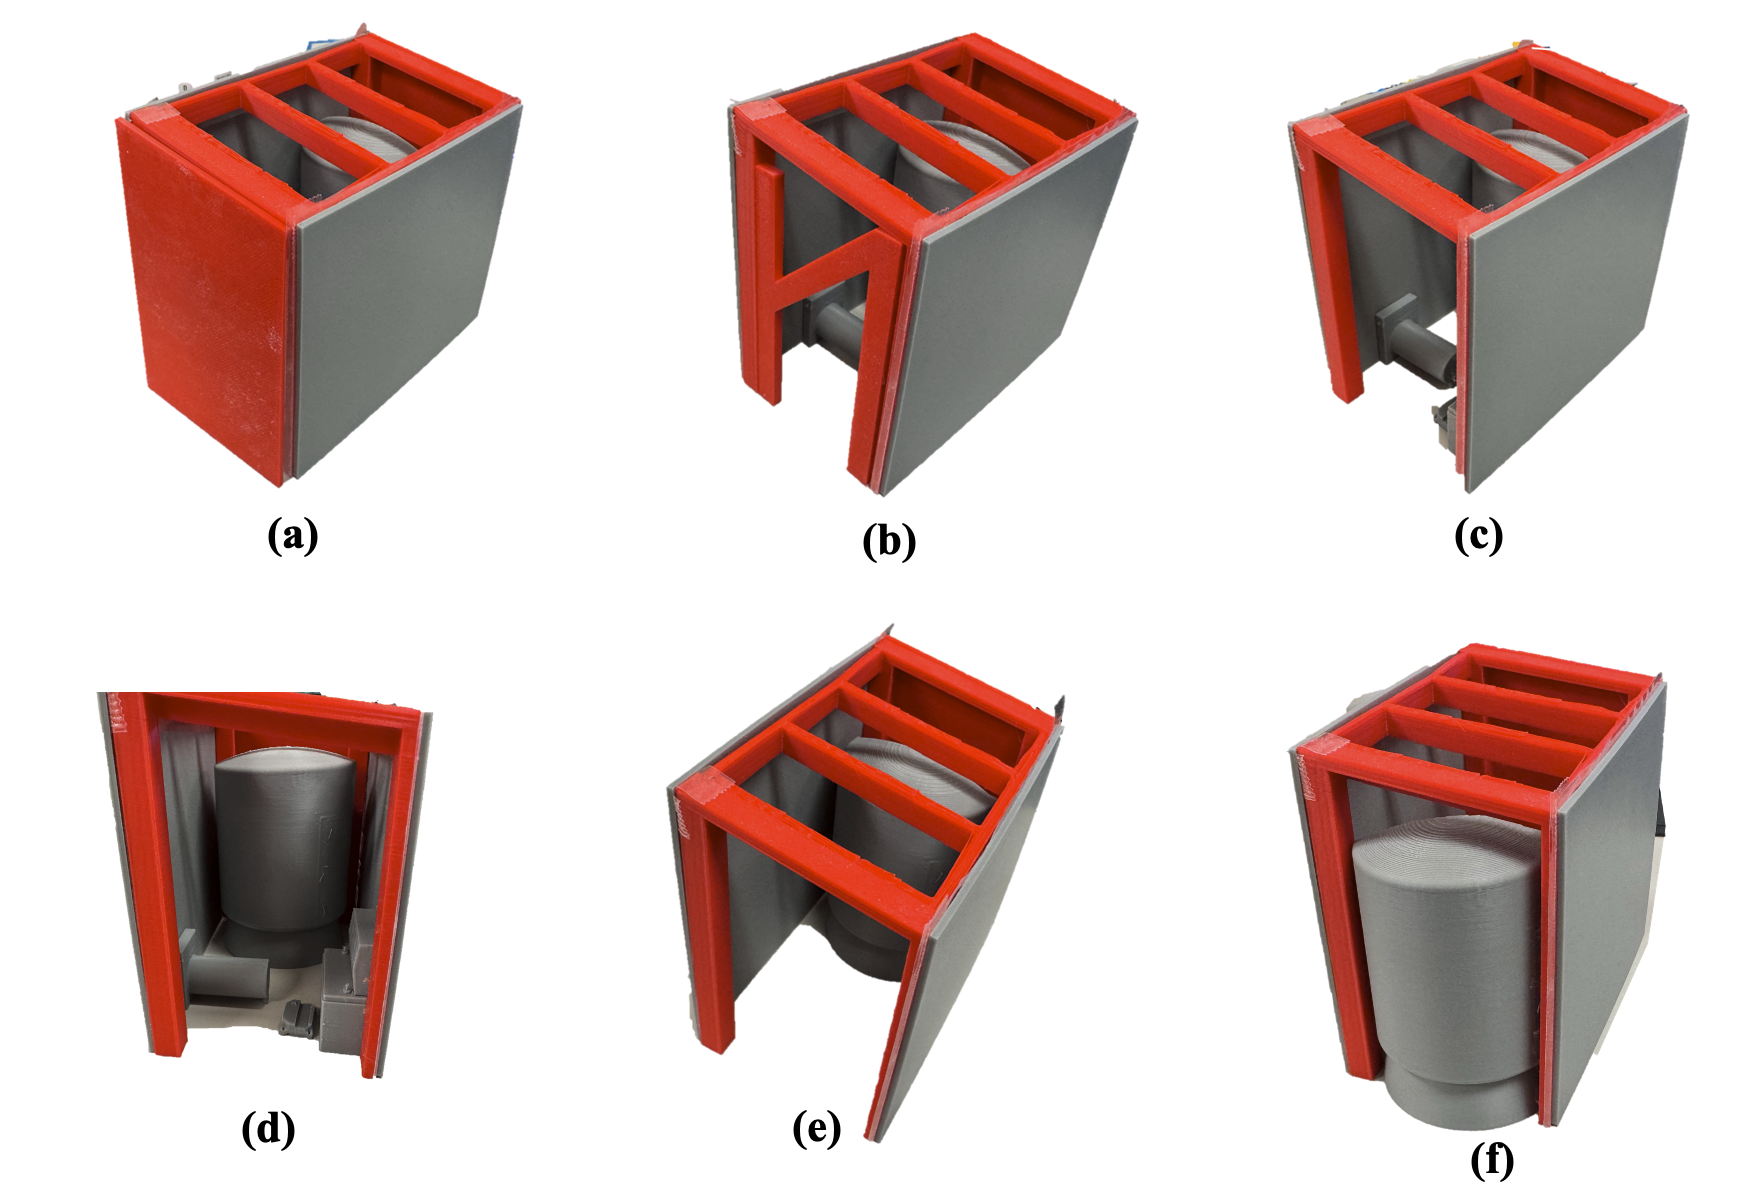
\includegraphics[width=\textwidth]{1.10 scale.png}
    \caption{1:10 scale mockup}
    \label{fig:mockup-photo10}
\end{figure}

\begin{figure}[H]
    \centering
    \rotatebox{270}{%
        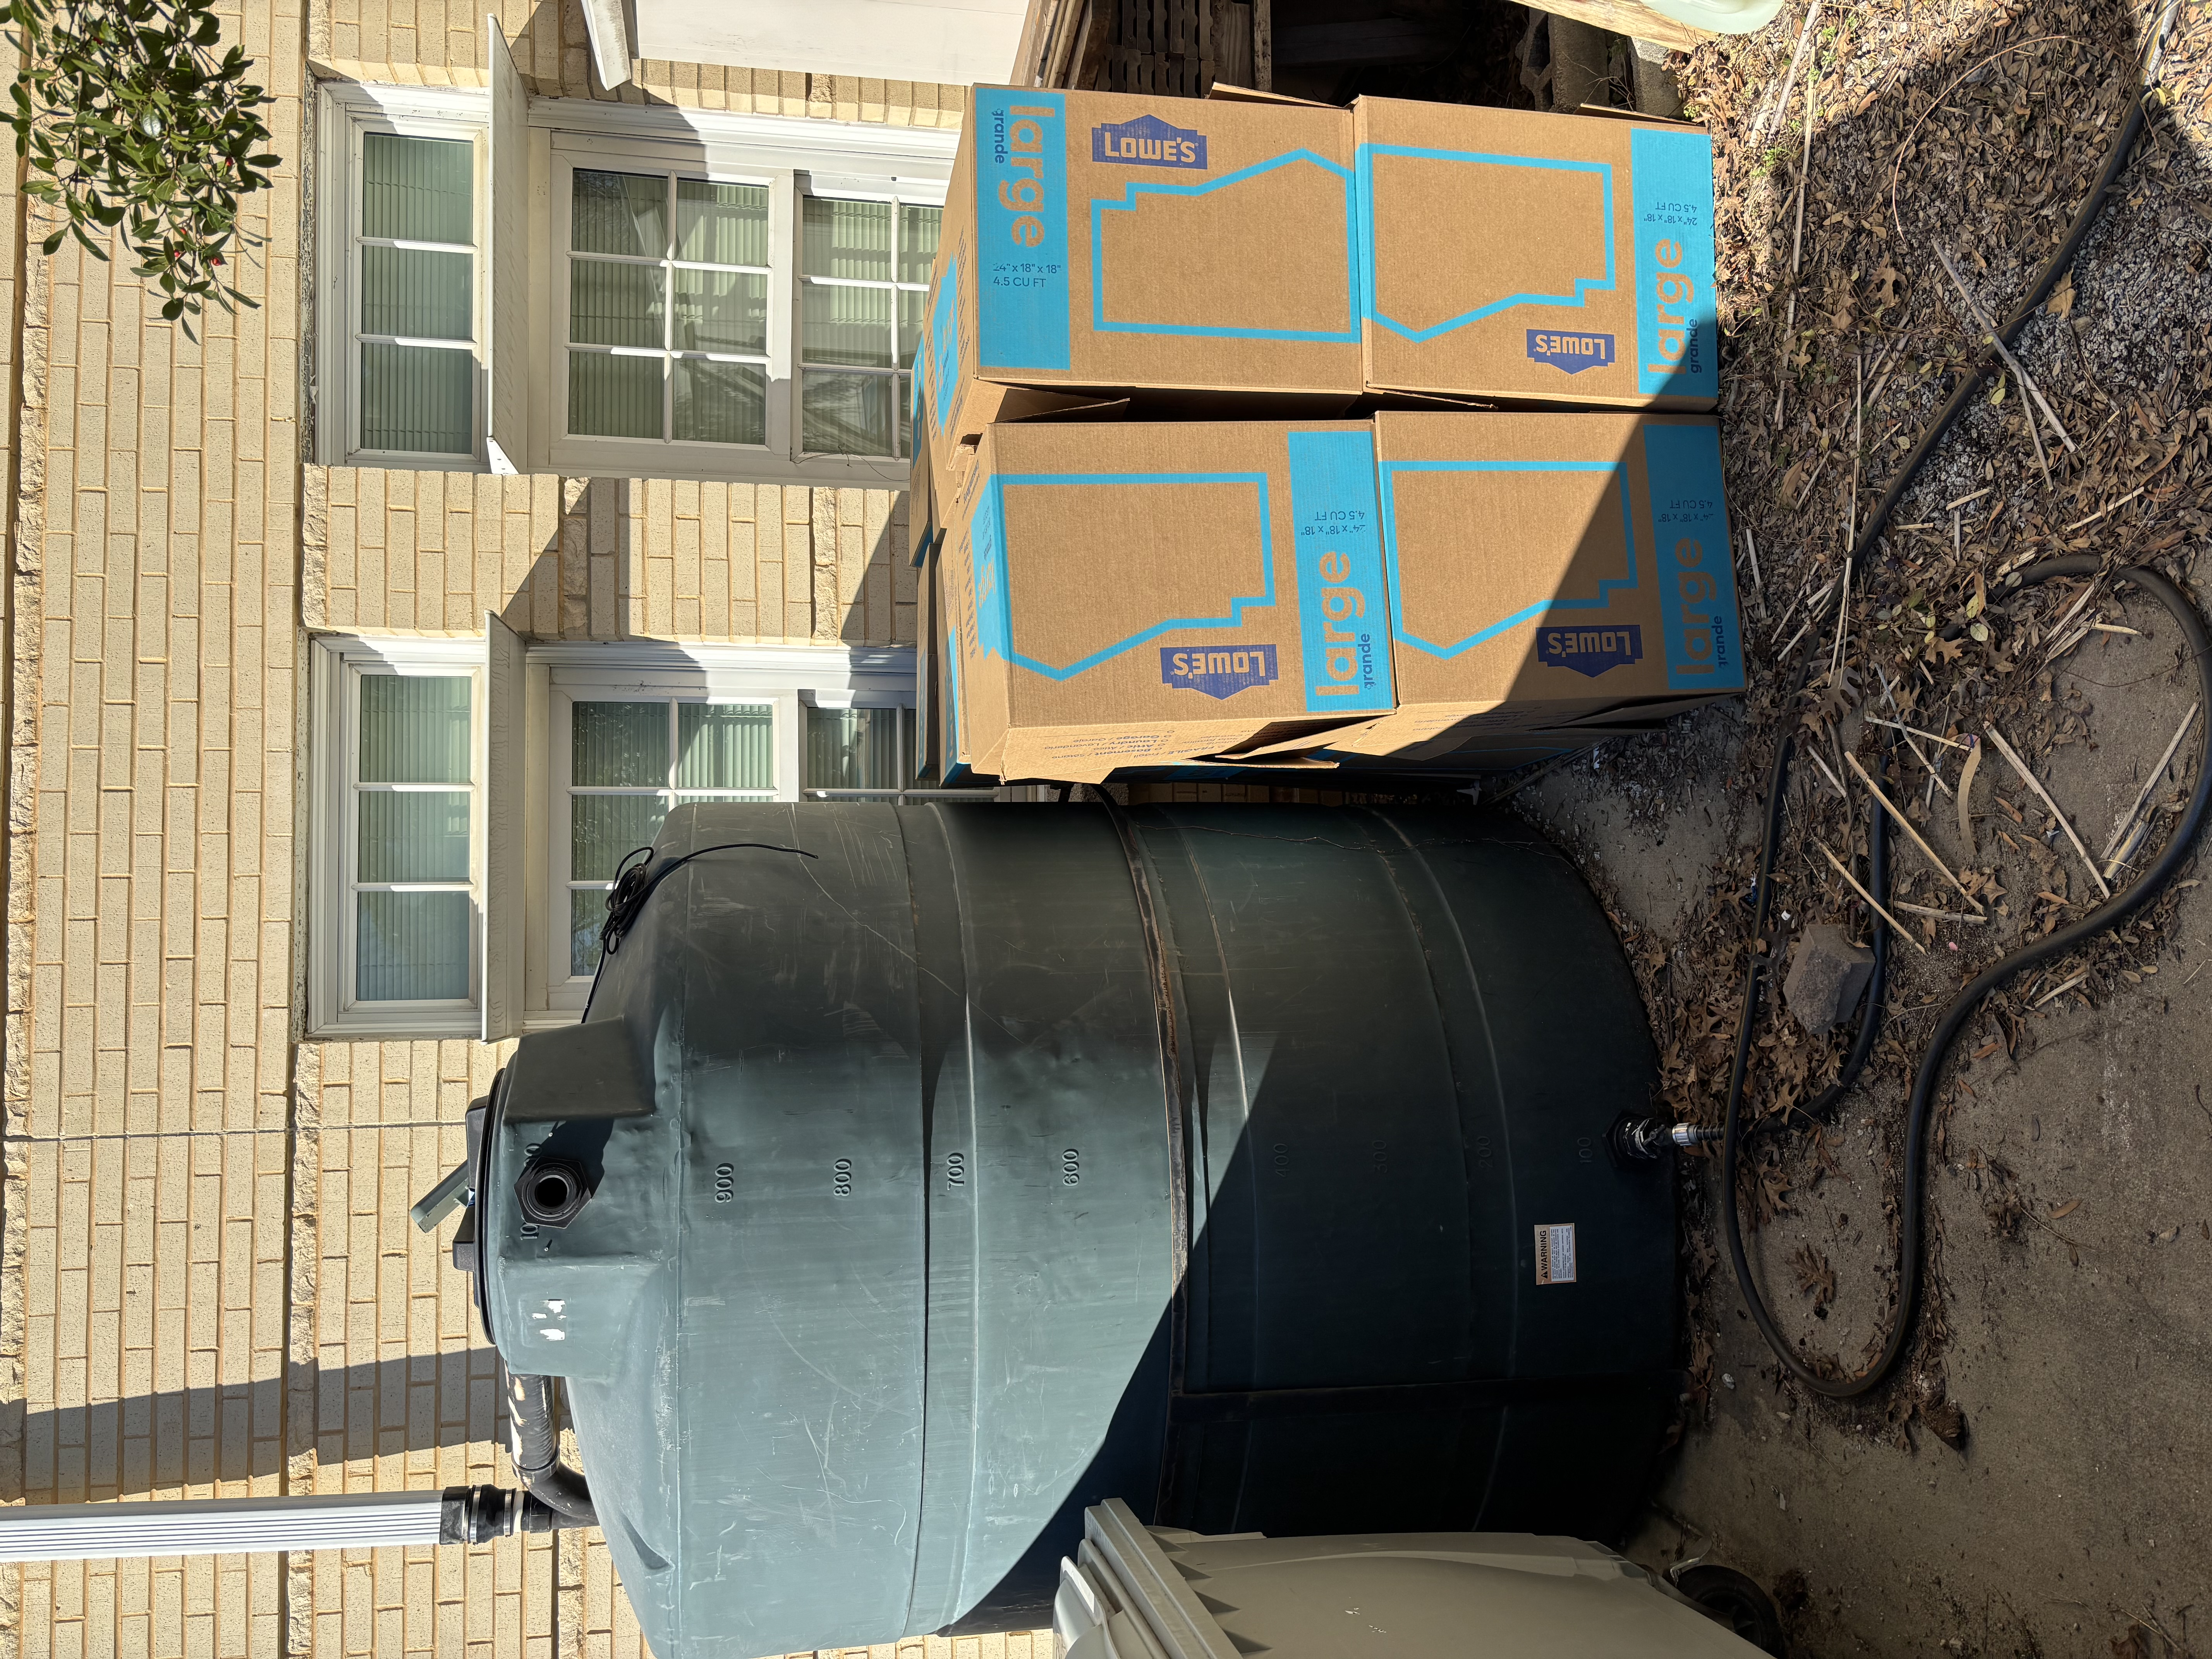
\includegraphics[width=\textwidth]{1.1 scale.jpeg}
    }
    \caption{1:1 scale mockup}
    \label{fig:mockup-photo1}
\end{figure}

\section{Lessons Learned}
\begin{enumerate}
    \item Some bracing may be required in the corners; however, this can be added during build-time.
    \item There will need to be additional bracing for the electronics mounting, or the placement for the electronics needs to be revised entirely.
    \item More fasteners will be required for the piping to reduce water hammer, especially given the use of plywood instead of deck planks.
    \item The build sequence will be modified. Instead of building the housing first, the pressurization system will be built(AC power), followed by the solar/DC system, and finally the housing will be constructed around these components. This change also necessitates careful placement of piping to reduce complications with hole placement.
\end{enumerate}

\section{Changes to Original Design}
\begin{enumerate}
    \item The concept will be mirrored to position the assembly on the left side of the tank instead of the right, reducing blockage of the window.
    \item The housing will be widened to allow for easier tank removal.
    \item Plywood will be used in place of decking planks. Plywood facilitates faster installation, and when painted, it protects against deterioration. This substitution also reduces the number of fasteners needed.
\end{enumerate}

\end{document}
